% !TEX root = saveliev_physics_general_course_2.tex
%!TEX TS-program = pdflatex
%!TEX encoding = UTF-8 Unicode


\chapter[DAO ĐỘNG ĐIỆN TỪ]{DAO ĐỘNG ĐIỆN TỪ}\label{chap:13}
\chaptermark{DAO ĐỘNG ĐIỆN TỪ}

\section{Dòng điện giả tĩnh}\label{sec:13_1}

Khi khảo sát các dao động điện từ, chúng ta phải tính toán với các dòng điện biến thiên.
Định luật Ohm và các định luật Kirchhoff chỉ có thể áp dụng cho các dòng điện không đổi theo thời gian.
Mặc dù vậy, chúng cũng có thể được dùng cho giá trị tức thời của dòng điện và điện áp biến thiên nếu các biến thiên này không quá nhanh.

Các nhiễu động điện từ truyền dọc theo mạch với tốc độ bằng tốc độ ánh sáng $c$.
Giả sử rằng độ dài của một đoạn mạch là $l$.
Nếu trong khoảng thời gian $\tau=l/c$ cần thiết để truyền các nhiễu động tới điểm xa nhất trên mạch, biến thiên dòng điện không đáng kể, thì khi đó giá trị tức thời của dòng điện tại mọi tiết diện trên mạch coi như là bằng nhau.
Dòng điện thỏa yêu cầu này được gọi là \textbf{giả tĩnh} (có thể coi là tĩnh - ND).
Với các dòng biến thiên tuần hoàn, điều kiện cho một trạng thái giả tĩnh là
\begin{equation*}
    \tau = \frac{l}{c} \ll T,
\end{equation*}

\noindent
với $T$ là chu kỳ biến thiên.

Độ trễ của một mạch dài \SI{3}{\metre} là $\tau=\SI{e-8}{\second}$.
Do đó với giá trị của $T$ đạt cỡ \SI{e-6}{\second} (tương đương tần số \SI{e6}{\hertz}), dòng điện trong một mạch như vậy có thể xem là giả tĩnh.
Dòng điện tần số điện lưới ($\nu= 50$ hoặc \SI{60}{\hertz}) được coi là giả tĩnh với các mạch dài lên tới \SI{100}{\kilo\metre}.

Giá trị tức thời của các dòng giả tĩnh tuân theo định luật Ohm.
Do đó, các định luật Kirchhoff cũng có thể áp dụng cho chúng.

Trong các phần sau khi nghiên cứu về dao động điện từ, ta luôn giả thiết rằng dòng điện đang tính toán là giả tĩnh.

\section{Dao động tự do trong mạch không điện trở}\label{sec:13_2}


Dao động điện từ có thể diễn ra ở một mạch gồm cuộn cảm và tụ điện.
Một mạch như vậy được gọi là \textbf{mạch dao động}.
Hình \ref{fig:13_1}a cho thấy các pha liên tiếp trong một quá trình dao động ở một mạch lý tưởng không có điện trở.

\begin{figure}[t]
	\begin{center}
		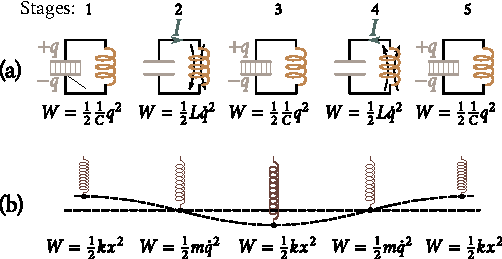
\includegraphics[scale=1.1]{figures/ch_13/fig_13_1.pdf}
		\caption[]{}
		\label{fig:13_1}
	\end{center}
	\vspace{-0.8cm}
\end{figure}

Dao động có thể được thiết lập bằng cách nạp một lượng điện tích đầu nhất định tới tụ hoặc đưa một một dòng vào cuộn cảm (chẳng hạn như bật tắt từ trường ngoài đi qua các vòng dây trên cuộn).
Ở đây ta xét cách thứ nhất.
Ta nối tụ tới một nguồn áp sau khi ngắt nó khỏi cuộn cảm.
Kết quả là sự xuất hiện điện tích trái dấu $+q$ and $-q$ trên các bản tụ (giai đoạn $1$).
Điều này sẽ thiết lập một điện trường giữa các bản tụ, và năng lượng hệ là $(q^2/C)/2$ [xem \eqn{4_5}].
Nesu ta ngắt nguồn áp và nối tụ vào cuộn cảm, tụ sẽ dần xả và dòng sẽ chạy qua mạch.
Năng lượng điện trường sẽ giảm đi, nhưng năng lượng từ trường do dòng chạy qua cuộn cảm sẽ tăng lên.
Năng lượng này là $LI^2/2$ [xem \eqn{8_37}].

Do điện trở cảu mạch bằng 0, tổng năng lượng bao gồm năng lượng điện trường và từ trường không chuyển sang nhiệt năng và sẽ giữ nguyên\footnote{Một cách chặt chẽ, ở một mạch lý tưởng, năng lượng sẽ bị mất do sự phát sóng điện từ. Sự thất thoát này sẽ tăng theo tần số dao động và khi mạch ``mở'' hơn}.
Do đó, tại thời điểm mà điện áp trên tụ, và theo đó là năng lượng điện trường giảm về không, năng lượng từ trường, và theo đó là dòng điện đạt giá trị cực đại (giai đoạn $2$; từ thời điểm này, dòng điện chạy dựa vào suất điện động tự cảm).
Sau đó, dòng điện giảm dần và khi điện tích trên tụ đạt giá trị ban đầu $q$, dòng điện sẽ về không (giai đoạn $3$).
Sau đó, quá trình này diễn ra với chiều ngược lại (giai đoạn $4$ và $5$).
Sau đó, hệ sẽ trở về trạng thái ban đầu (giai đoạn $5$), và vòng lặp này sẽ lặp đi lặp lại.
Điện tích trên tụ, điện áp trên tụ và dòng chạy trong cuộn cảm biến thiên điều hòa (\ie, dao động) trong suốt chu trình này.
Dao động này còn đi kèm sự biến thiên đồng thời của năng lượng điện trường và từ trường.

Hình \ref{fig:13_1}b thể hiện sự tương đồng của dao động lò xo và của mạch LC.
Việc nạp điện cho tụ tương đương với việc kéo con lắc khỏi vị trí cân bằng một đoạn $x$ bằng cách tác dụng ngoại lực.
Việc này truyền thế năng biến dạng đàn hồi của lò xo bằng $kx^2/2$.
Giai đoạn 2 tương ứng với con lắc đi qua vị trí cân bằng.
Tại thời điểm này, lực giả-đàn hồi bằng không và con lắc tiếp tục chuyển động nhờ quán tính.
Tại thời điểm này, năng lượng của con lắc chuyển hoàn toàn thành động năng với giá trị bằng biểu thức $m\dot{x}^2/2$.
Độc giả có thể tiếp tục so sánh các giai đoạn sau đó.

Có thể thấy sự tương đương của dao động điện từ và cơ học ở chỗ năng lượng điện trường $q^2/2C$ tương tự với thế năng đàn hồi, và năng lượng điện từ $LI^2$ tương đương với động nawgn.
Độ tự cảm $L$ đóng vai trò của khối lượng $m$ và nghịch đảo của điện dung $(1/C)$ đóng vai trò của độ cứng lò xo $k$.
Sau cùng, độ dời của con lắc từ vị trí cân bằng $x$ tương ứng với điện tích $q$, và tốc độ $\dot{x}$ tương ứng với dòng điện $I = \dot{q}$.
Ta thấy rằng sự tương ứng giữa dao động điện từ và cơ học cũng trải đến các phương trình toán học biểu diễn chúng.

Ta đi tìm phương trình cho mạch không có điện trở (mạch $L$-$C$ circuit).
Quy ước dấu cho dòng nạp tụ là dương\footnote{Với lựa chọn này, sự tương tự giữa dao động điện và cơ sẽ hoàn chỉnh hơn: $\dot{q}$ tương đương với tốc độ $\dot{X}$ (khi chọn chiều khác, $-\dot{q}$ tương đương với tốc độ $\dot{x}$).} (\fig{13_2}).
Do đó, từ \eqn{5_1},
\begin{equation*}
    I = \diff{q}{t} = \dot{q}.
\end{equation*}

\begin{figure}[t]
	\begin{center}
		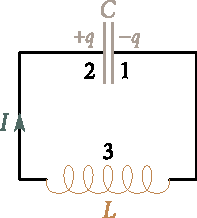
\includegraphics[scale=1]{figures/ch_13/fig_13_2.pdf}
		\caption[]{}
		\label{fig:13_2}
	\end{center}
	\vspace{-0.8cm}
\end{figure}

\noindent
Phương trình \eqref{eq:5_27} của định luật Ohm cho mạch $1$-$3$-$2$ là
\begin{equation*}
    IR = \varphi_1 - \varphi_2 + \mathcal{E}_{12}.
\end{equation*}

\noindent
Trong trường hợp này, $R=0$, $\varphi_1 - \varphi_2=-q/C$, và $\mathcal{E}_{12}=\ab{\mathcal{E}}{s} = -L\, (\diffin{I}{t})$.
Thế các giá trị này vào \eqn{5_27}, ta nhận
\begin{equation}\label{eq:13_1}
    0 = - \frac{q}{C} - L\, \diff{I}{t}.
\end{equation}

\noindent
Cuối cùng, thế $\diffin{I}{t}$ bằng $\ddot{q}$ [xem \eqn{5_1}], ta có
\begin{equation}\label{eq:13_2}
    \ddot{q} + \frac{1}{LC} q = 0.
\end{equation}

Ta ký hiệu
\begin{equation}\label{eq:13_3}
    \omega_0 = \frac{1}{\sqrt{LC}},
\end{equation}

\noindent
\eqn{13_2} trở thành
\begin{equation}\label{eq:13_4}
    \ddot{q} + \omega_0^2 q = 0,
\end{equation}

\noindent
một công thức quen thuộc từ phần dao động cơ học [xem Eq. (7.7) của Tập I].
Hàm sau đây là một nghiệm của phương trình này
\begin{equation}\label{eq:13_5}
    q = \ab{q}{m} \cos(\omega_0 t + \alpha)
\end{equation}

\noindent
(ký tự dưới ``m'' đại diện cho tối đa (maximum)).

Do đó, điện tích trên các bản tụ biến thiên điều hòa với tần số được cho bởi \eqn{13_3}.
Tần số này được gọi là \textbf{tần số riêng của mạch} (tương ứng với tần số riêng của một dao động điều hòa).
Chúng ta có được \textbf{công thức Thomson} cho chu kỳ dao động.
\begin{equation}\label{eq:13_6}
    T = \frac{2\pi}{\sqrt{LC}}.
\end{equation}

Điện áp trên tụ khác điện tích một hệ số $1/C$:
\begin{equation}\label{eq:13_7}
    U = \frac{\ab{q}{m}}{C} \cos(\omega_0 t + \alpha) = \ab{U}{m} \cos(\omega_0 t + \alpha).
\end{equation}

Đạo hàm thời gian của \eqn{13_5} đưa lại biểu thức của dòng điện:
\begin{equation}\label{eq:13_8}
    I = - \omega_0 \ab{q}{m} \sin(\omega_0 t + \alpha) = \ab{I}{m} \cos(\omega_0 t + \alpha + \frac{\pi}{2}).
\end{equation}

\noindent
Do đó, dòng điện sớm pha $\pi/2$ hơn so với điện áp trên tụ.

Khi đối chiếu \eqns{13_5}{13_7} với \eqn{13_8} ta thấy rằng khi dòng điện đạt giá trị cực đại, điện áp và điện tích biến mất và ngược lại.
Chúng ta đã thiết lập được liên hệ giữa điện áp và dòng điện khi xem xét năng lượng của hệ.

Khảo sát \eqns{13_7}{13_8} ta thấy
\begin{equation*}
    \ab{U}{m} = \frac{\ab{q}{m}}{C}, \quad \ab{I}{m} = \omega_0 \ab{q}{m}.
\end{equation*}

\noindent
Ta tìm tỉ số của các biên độ này và thế giá trị $\omega_0$ từ \eqn{13_3}, ta có
\begin{equation}\label{eq:13_9}
    \ab{U}{m} = \parenthesis{\frac{L}{C}}^{1/2}\, \ab{I}{m}.
\end{equation}

\noindent
Chúng ta cũng có thể tìm được liên hệ này nếu nhận ra rằng giá trị cực đại của năng lượng điện trường $C\ab{U}{m}^2/2$ phải bằng giá trị cực đại của năng lượng điện từ $L\ab{I}{m}^2/2$.

\section{Dao động tắt dần tự do}\label{sec:13_3}

Bất kỳ mạch thực tế nào đều có điện trở.
Năng lượng trữ trong mạch được điện trở này biến thành nhiệt, do đó mà dao động tự do trở thành tắt dần.


Phương trình \eqref{eq:5_27} cho mạch $1$-$3$-$2$ tại \fig{13_3} có dạng
\begin{equation}\label{eq:13_10}
    IR = - \frac{q}{C} - L\, \diff{I}{t}
\end{equation}

[so với \eqn{13_1}].
Chia phương trình này cho $L$ và thế $\dot{q}$ cho $I$ và  $\ddot{q}$ cho $\diffin{I}{t}$, ta nhận được
\begin{equation}\label{eq:13_11}
    \ddot{q} + \frac{R}{L}\, \dot{q} + \frac{1}{LC}\, q = 0.
\end{equation}

\begin{figure}[t]
	\begin{center}
		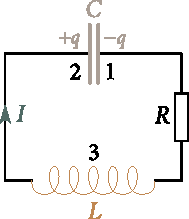
\includegraphics[scale=1]{figures/ch_13/fig_13_3.pdf}
		\caption[]{}
		\label{fig:13_3}
	\end{center}
	\vspace{-0.8cm}
\end{figure}

Khi tính đến việc nghịch đảo của $LC$ bằng bình phương tần số tự nhiên của mạch $\omega_0$ [xem \eqn{13_3}], và đặt ký hiệu
\begin{equation}\label{eq:13_12}
    \beta = \frac{R}{LC},
\end{equation}

\noindent
\eqn{13_11} có thể được viết dưới dạng
\begin{equation}\label{eq:13_13}
    \ddot{q} + 2 \beta \dot{q} + \omega_0^2 q = 0.
\end{equation}

Phương trình này có dạng tương đương với phương trình vi phân của dao động tắt dần cơ học [xem Eq. (7.11) tại Tập I].

Khi $\beta^2<\omega_0^2$, \ie, $R^2/(4L^2)<1/(LC)$, nghiệm \eqn{13_3} có dạng
\begin{equation}\label{eq:13_14}
    q = \ab{q}{m,$0$}\, e^{-\beta t} \cos(\omega t + \alpha),
\end{equation}

\noindent
với $\omega=\sqrt{\omega_0^2-\beta^2}$.
Thế giá trị cho $\omega_0$ từ \eqn{13_3} và $\beta$ từ \eqn{13_12}, ta được
\begin{equation}\label{eq:13_15}
    \omega = \parenthesis{ \frac{1}{LC} - \frac{R^2}{4L^2} }.
\end{equation}

\noindent
Do đó tần số của dao động tắt dần $\omega$ nhỏ hơn tần số tự nhiên $\omega_0$.
Khi  $R=0$, \eqn{13_13} trở thành \eqn{13_3}.

Chia \eqn{13_14} cho điện dung $C$, ta có điện áp rơi trên tụ:
\begin{equation}\label{eq:13_16}
    U = \frac{1}{C} \ab{q}{m,$0$}\, e^{-\beta t} \cos(\omega t + \alpha) = \ab{U}{m,$0$}\, e^{-\beta t} \cos(\omega t + \alpha).
\end{equation}

Để tìm dòng điện, ta đạo hàm \eqn{13_14} theo thời gian
\begin{equation*}
    I = \dot{q} = \ab{q}{m,$0$}\, e^{-\beta t} [-\beta \cos(\omega t + \alpha) - \omega \sin(\omega t + \alpha)].
\end{equation*}

\noindent
Nhân vế phải của phương trình này bằng biểu thức
\begin{equation*}
    \frac{\omega_0}{\sqrt{\omega^2-\beta^2}}
\end{equation*}

\noindent
bằng một, ta được
\begin{equation*}
    I = \omega_0 \ab{q}{m,$0$}\, e^{-\beta t} \bracket{ - \frac{\beta}{\sqrt{\omega^2-\beta^2}} \cos(\omega t + \alpha) - \frac{\omega}{\sqrt{\omega^2-\beta^2}} \sin(\omega t + \alpha) }.
\end{equation*}

Đặt góc $\psi$ xác định bởi điều kiện
\begin{equation*}
    \cos\psi = - \frac{\beta}{\sqrt{\omega^2-\beta^2}} = - \frac{\beta}{\omega_0},\quad \sin\psi = \frac{\omega}{\sqrt{\omega^2-\beta^2}} = \frac{\omega}{\omega_0},
\end{equation*}

\noindent
ta có thể viết
\begin{equation}\label{eq:13_17}
    I = \omega_0 \ab{q}{m,$0$}\, e^{-\beta t} \cos(\omega t + \alpha + \psi).
\end{equation}

\noindent
Do $\cos\psi<0$ và $\sin\psi>0$, giá trị của $\psi$ nằm trong khoảng từ $\pi/2$ đến $\pi$ (\ie, $\pi/2<\psi<\pi$).
Do đó khi một mạch chứa điện trở, dòng điện sớm pha so với điện áp trên tụ hơn $\pi/2$ (khi $R=0$, độ lệch pha là $\pi/2$).

Một đồ thị của hàm \eqref{eq:13_14} được biểu diễn tại \fig{13_4}.
Đồ thị của điện áp và dòng điện đều tương tự.

Thông thường ta sử dụng \textbf{độ giảm loga} để đặc trưng cho độ hãm dao động.
\begin{equation}\label{eq:13_18}
    \lambda = \ln\bracket{ \frac{A(t)}{A(t+T)} } = \beta T
\end{equation}

\noindent
[xem phương trình (7.104) tại Tập I].
Với $A(t)$ là biên độ của đại lượng khảo sát ($q$, $U$, or $I$).
Ta lưu ý rằng độ giảm loga là nghịch đảo của số dao động $N_e$ diễn ra trong khoảng thời gian cần thiết để biên độ giảm đi $1/e$ giá trị ban đầu:
\begin{equation*}
    \lambda = \frac{1}{N_e}.
\end{equation*}

\begin{figure}[t]
	\begin{center}
		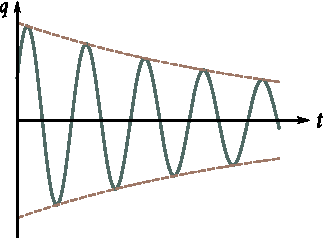
\includegraphics[scale=1]{figures/ch_13/fig_13_4.pdf}
		\caption[]{}
		\label{fig:13_4}
	\end{center}
	\vspace{-0.8cm}
\end{figure}

Thay giá trị $\beta$ từ \eqn{13_12} vào \eqn{13_18} và thay $2\pi/\omega$ cho $T$, ta có biểu thức cho $A$:
\begin{equation}\label{eq:13_19}
    \lambda = \frac{R}{2L} \frac{2\pi}{\omega} = \frac{\pi R}{L\omega}.
\end{equation}

\noindent
Tần số $\omega$, và qua đó, $A$ được xác định bởi các tham số của mạch $L$, $C$, and $R$.
Do đó, độ giảm loga là một đại lượng đặc trưng của mạch

Nếu độ hãm nhỏ ($\beta^2\ll\omega_0^2$), ta có giả thiết tại \eqn{13_19} rằng $\omega\approx\omega_0 = 1/\sqrt{LC}$.
Từ đó,
\begin{equation}\label{eq:13_20}
    \lambda \approx \frac{\pi R \sqrt{LC}}{L} = \pi R \parenthesis{\frac{C}{L}}^{1/2}.
\end{equation}

Một mạch dao động được trưng bởi phẩm chất của mạch, ký hiệu bởi $Q$, xác định bởi nghịch đảo của độ giảm loga.
\vspace{-12pt}
\begin{equation}\label{eq:13_21}
    Q = \frac{\pi}{\lambda} = \pi N_e.
\end{equation}

\noindent
Từ \eqn{13_21} ta thấy được phẩm chất của mạch càng cao thì số lần dao động thực hiện được trước khi biên độ giảm đi $1/e$ giá trị đầu của nó.

Với độ hãm yếu, ta có
\begin{equation}\label{eq:13_22}
    Q = \frac{1}{R} \parenthesis{\frac{L}{C}}^{1/2}
\end{equation}

\noindent
[xem \eqn{13_20}].

Tại phần 7.10 của Tập I, ta thấy rằng khi độ hãm yếu, phẩm chất của một hệ dao động cơ học bằng tỉ số giữa năng lượng của hệ tại thời điểm khảo sát với độ giảm năng lượng trong một chu kỳ dao động nhân với hệ số $2\pi$.
Ta chứng minh rằng điều này vẫn đúng với dao động điện từ.
Biên độ của dòng trong mạch giảm dần theo quy luật $e^{-\beta t}$.
Năng lượng $W$ trữ trong mạch tỉ lệ với bình phương biên độ dòng điện (hoặc bình phương biên độ điện áp trên tụ).
Do đó $W$ giảm dần theo quy luật $e^{-2\beta t}$.
Độ giảm năng lượng tương đối trong một chu kỳ là
\begin{equation*}
    \frac{\Delta{W}}{W} = \frac{W(t) - W(t+T)}{W(t)} = \frac{1 - e^{-2\beta t}}{1} = 1 - e^{-2\lambda}.
\end{equation*}

\noindent
Khi độ hãm nhỏ (\ie, when $A\ll 1$), ta có thể giả thiết rằng $e^{-2\lambda}$ xấp xỉ $1-2\lambda$:
\begin{equation*}
    \frac{\Delta{W}}{W} = 1 - (1 - 2\lambda) = 2 \lambda.
\end{equation*}

\noindent
Thế giá trị phẩm chất $Q$ của mạch vào $\lambda$ tại biểu thức này theo \eqn{13_21} và giải phương trình nhận được theo $Q$, ta được
\begin{equation}\label{eq:13_23}
    Q = 2\pi \frac{\Delta{W}}{W}.
\end{equation}

Lưu ý rằng khi $R^2/(4L^2)\geqslant 1/(LC)$, \ie, tức là $\beta^2\geqslant\omega_0^2$, ta có sự xả tụ không theo chu kỳ thay vì dao động.
Giá trị của điện trở mạch tại đó quá trình dao động chuyển thành không dao động được gọi là giá trị \textbf{tới hạn}.
Giá trị điện trở tới hạn $\ab{R}{cr}$ được xác định bởi điều kiện $\ab{R}{cr}^2/(4L^2)= 1/(LC)$, với
\begin{equation}\label{eq:13_24}
    \ab{R}{cr} = 2 \parenthesis{\frac{L}{C}}^{1/2}.
\end{equation}

\section{Dạo động điện từ cưỡng bức}\label{sec:13_4}

Để thực hiện dao động cưỡng bức lên hệ, phải có một tác động biến thiên điều hòa lên hệ.
Ta có thể thực hiện với dao động điện từ nếu nối tiếp một suất điện động biến thiên với các phần tử mạch, hoặc nếu sau khi đóng mạch, ta đưa một nguồn điện xoay chiều vào mạch \ie, điện áp
\begin{equation}\label{eq:13_25}
    U = \ab{U}{m} \cos(\omega t)
\end{equation}

\noindent
(\fig{13_5}).
Điện áp này phải được thêm vào suất điện động tự cảm của mạch.
Do đó, \eqn{13_10} có dạng
\begin{equation}\label{eq:13_26}
    IR = - \frac{q}{C} - L\, \diff{I}{t} + \ab{U}{m} \cos(\omega t).
\end{equation}

\noindent
Sau khi biến đổi, ta được phương trình
\begin{equation}\label{eq:13_27}
    \ddot{q} + 2\beta \dot{q} + \omega_0^2 q = \frac{\ab{U}{m}}{L} \cos(\omega t).
\end{equation}

\noindent
Với $\omega_0^2$ và $\beta$ được xác định bởi \eqns{13_3}{13_12}.

\begin{figure}[t]
	\begin{center}
		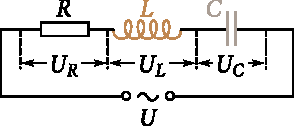
\includegraphics[scale=1]{figures/ch_13/fig_13_5.pdf}
		\caption[]{}
		\label{fig:13_5}
	\end{center}
	\vspace{-0.8cm}
\end{figure}

Phương trình \eqref{eq:13_27} tương ứng với phương trình vi phân dao động cơ học cưỡng bức [xem phương trình (7.111) tại Tập I].
Một nghiệm riêng của phương trình có dạng
\begin{equation}\label{eq:13_28}
    q = \ab{q}{m} \cos(\omega t - \psi),
\end{equation}

\noindent
với
\begin{equation*}
    \ab{q}{m} = \frac{\ab{U}{m}/L}{\sqrt{\parenthesis{\omega_0^2-\omega^2}^2 + 4\beta^2\omega^2}},\quad \tan\psi = \frac{2\beta\omega}{\omega_0^2-\omega^2}
\end{equation*}

\noindent
[xem phương trình (7.119), Tập I].
Thế giá trị của chúng vào $\omega_0$ và $\beta$ ta được
\begin{align}
    \ab{q}{m} &= \frac{\ab{U}{m}}{\omega \sqrt{R^2 + [\omega L - 1/(\omega C)]^2}},\label{eq:13_29}\\
    \tan\psi &= \frac{R}{[1/(\omega C) - \omega L]}.\label{eq:13_30}
\end{align}

Ta được nghiệm tổng quát khi thêm nghiệm tổng quát của phương trình thuần nhất tương ứng này vào nghiệm riêng \eqref{eq:13_28}.
Nghiệm này được tìm ở phần trước [\eqn{13_14}].
Nó chứa thành phần lũy thừa $e^{-\beta t}$, do đó, sau một quãng thời gian đủ lớn, trở nên rất nhỏ và có thể bỏ qua.
Từ đó, dao động cưỡng bức tĩnh được biểu diễn bởi hàm \eqref{eq:13_28}.

Đạo hàm của \eqn{13_28} cho ta dòng điện trong mạch với dao động tĩnh:
\begin{equation*}
    I = -\omega \ab{q}{m} \sin(\omega t - \psi) = \ab{I}{m} \cos\parenthesis{ \omega t - \psi + \frac{\pi}{2} }
\end{equation*}

\noindent
($\ab{I}{m}=\omega\ab{q}{m}$).
Ta có thể viết biểu thức này dưới dạng \footnote{Ta sẽ không gặp khái niệm điện thế cho đến hết chương này. Do đó có thể tùy ý sử dụng ký hiệu $\varphi$ cho góc pha}
\begin{equation}\label{eq:13_31}
    I = \ab{I}{m} \cos(\omega t - \varphi),
\end{equation}

\noindent
với $\varphi=\psi-\pi/2$ là độ lệch pha giữa dòng điện và điện áp [tham khảo \eqn{13_25}].
Theo \eqn{13_30}:
\begin{equation}\label{eq:13_32}
    \tan\varphi = \tan\parenthesis{\psi - \frac{\pi}{2}} = - \frac{q}{\tan\psi} = \frac{\omega L - 1/(LC)}{R}.
\end{equation}

\noindent
Khảo sát phương trình này cho thấy dòng điện trễ pha so với điện thế ($\varphi>0$) khi $\omega L>1/(\omega C)$, và sớm pha  ($\varphi<0$) khi $\omega L<1/(\omega C)$.
Theo \eqn{13_29}:
\begin{equation}\label{eq:13_33}
    \ab{I}{m} = \omega \ab{q}{m} = \frac{\ab{U}{m}}{\sqrt{R^2 + [\omega L - 1/(\omega C)]^2}}.
\end{equation}

\noindent
Có thể viết \eqn{13_26} dưới dạng
\begin{equation}\label{eq:13_34}
    IR + \frac{q}{C} + L\, \diff{I}{t} = \ab{U}{m} \cos(\omega t).
\end{equation}

\noindent
Tích $IR$ bằng điện áp $U_R$ rơi trên tụ, $q/C$ là điện áp trên $U_C$, và biểu thức $L\,(\diffin{I}{t})$ xác định điện áp trên cuộn cảm $U_L$.
Từ đây có thể viết
\begin{equation}\label{eq:13_35}
    U_R + U_C + U_L = \ab{U}{m} \cos(\omega t).
\end{equation}

\noindent
Do đó, tổng điện áp dọc các phần tử mạch tại mọi thời điểm bằng điện áp cấp từ nguồn (theo \fig{13_5}).

Từ \eqn{13_31} ta có
\begin{equation}\label{eq:13_36}
    U_R = R \ab{I}{m} \cos(\omega t - \varphi).
\end{equation}

\noindent
Chia \eqn{13_28} cho điện dung, ta có điện áp trên tụ
\begin{equation}\label{eq:13_37}
    U_C = \frac{\ab{q}{m}}{C} \cos(\omega t - \psi) = \ab{U}{$C$,m} \cos\parenthesis{\omega t - \varphi - \frac{\pi}{2}}.
\end{equation}

\noindent
Tại đây
\begin{equation}\label{eq:13_38}
    \ab{U}{$C$,m} = \frac{\ab{q}{m}}{C}  = \frac{\ab{U}{m}}{\omega C \sqrt{R^2 + [\omega L - 1/(\omega C)]^2}} = \frac{\ab{I}{m}}{\omega C}
\end{equation}

\noindent
[see \eqn{13_31}].
Nhân đạo hàm của \eqref{eq:13_31} với $L$, ta có điện áp trên cuộn cảm:
\begin{equation}\label{eq:13_39}
    U_L = L\, \diff{I}{t} = - \omega L \ab{I}{m} \sin(\omega t - \varphi) = \ab{U}{$L$,m} \cos\parenthesis{\omega t - \varphi + \frac{\pi}{2}}.
\end{equation}

\noindent
Ta có
\begin{equation}\label{eq:13_40}
    \ab{U}{$L$,m} = \omega L \ab{I}{m}.
\end{equation}

Đối chiếu giữa các phương trình \eqref{eq:13_31}, \eqref{eq:13_36}, \eqref{eq:13_37}, và \eqref{eq:13_39} ta thấy điện áp trên tụ trễ so với dòng điện một pha $pi/2$, trong khi đó điện áp trên cuộn cảm sớm so với dòng điện một pha $pi/2$. Điện áp trên điện trở biến thiên đồng pha với dòng điện. 
Các mối liên hệ này có thể được thể hiện bằng một sơ đồ vector (xem Phần 7.7, tập I).
Ta biết rằng một dao động điều hòa (hoặc một hàm điều hòa) có thể được biểu diễn dưới dạng một vector với chiều dài bằng biên độ dao động, với hướng của vector tạo góc bằng với pha ban đầu với một trục cho trước.
Ta chọn trục của dòng điện là gốc tính pha ban đầu.
Ta được sơ đồ tại \fig{13_6}.

\begin{figure}[t]
	\begin{center}
		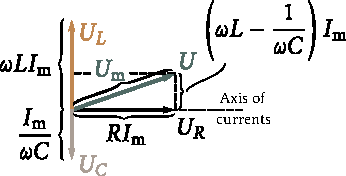
\includegraphics[scale=1]{figures/ch_13/fig_13_6.pdf}
		\caption[]{}
		\label{fig:13_6}
	\end{center}
	\vspace{-0.8cm}
\end{figure}

\noindent
Dựa theo \eqn{13_35}, tổng của ba hàm $U_R$, $U_C$, and $U_L$ phải bằng điện áp nguồn $U$.
Do đó điện áp $U$ được biểu diễn bởi vector bằng tổng của các vector $U_R$, $U_C$, and $U_L$.
Lưu ý rằng \eqn{13_33} có thể rút ra dễ dàng từ tam giác vuông tại biểu đồ vector có các cạnh $U$, $U_R$ và hiệu  $U_L-U_C$.

Tần số cộng hưởng cho điện tích $q$ và điện áp $U_C$ trên tụ là
\begin{equation}\label{eq:13_41}
    \ab{\omega}{$q$,res} = \ab{\omega}{$U$,res} = \parenthesis{\omega_0^2 - 2\beta^2}^{1/2} = \parenthesis{\frac{1}{LC} - \frac{R^2}{2L^2}}^{1/2}\leqslant \omega_0
\end{equation}

\noindent
[theo phương trình (7.127), Tập I].

Đường cong cộng hưởng cho $U_C$ được cho tại \fig{13_7} (đường cong cộng hưởng $q$ có chung dạng).
Chúng tương tự với đường cong cộng hưởng cho dao động cơ học (xem Hình 7.24 tập I).
Khi $\omega\to 0$, đường cong cộng hưởng hội tụ tại điểm có tọa độ $\ab{U}{$C$,m}=\ab{U}{m}$, \ie, điện áp trên tụ khi nó được nối đến nguồn điện áp không đổi $\ab{U}{m}$.
Cực đại cộng hưởng sẽ cao hơn và nhọn hơn khi $\beta=R/(2L)$ nhỏ hơn, \ie, điện trở nhỏ đi và điện cảm cao hơn.

Đường cong cộng hưởng cho dòng điện được cho tại \fig{13_8}.
Chúng tương ứng với đường cong cộng hưởng cho vận tốc trong dao động cơ học.
Biên độ dòng đạt giá trị cực đại tại
$\omega L - 1/(\omega C)$ [theo \eqn{13_33}]. Do đó, tần số cộng hưởng của dòng điện trùng với tần số tự nhiên của mạch $\omega_0$:
\begin{equation}\label{eq:13_42}
    \ab{\omega}{$I$,res} = \omega_0 = \frac{1}{\sqrt{LC}}.
\end{equation}

\begin{figure}[t]
	\begin{minipage}[t]{0.48\linewidth}
		\begin{center}
			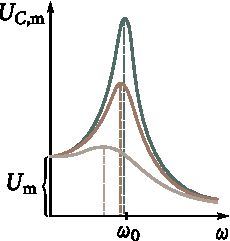
\includegraphics[scale=1]{figures/ch_13/fig_13_7.pdf}
			\caption[]{}
			\label{fig:13_7}
		\end{center}
	\end{minipage}
	\hfill{ }%space{-0.05cm}
	\begin{minipage}[t]{0.48\linewidth}
		\begin{center}
			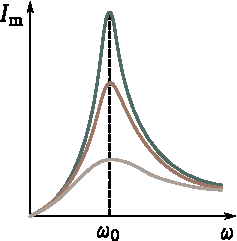
\includegraphics[scale=1]{figures/ch_13/fig_13_8.pdf}
			\caption[]{}
			\label{fig:13_8}
		\end{center}
	\end{minipage}
\vspace{-0.4cm}
\end{figure}

Giao điểm của đường cong cộng hưởng trên trục $I_m$ là bằng không--tại điện áp không đổi, một dòng ổn định không thể chạy trong mạch chứa tụ.

Khi hệ số cản nhỏ (khi $\beta^2\ll\omega_0^2$), tần số cộng hưởng cho điện áp có thể xem như là $\omega_0$ [see \eqn{13_41}].
Từ đó ta có thể xem tần số này như $\ab{\omega}{res}L-1/(\ab{\omega}{res}C)$.
Từ \eqn{13_38}, tỉ số giữa biên độ điện áp trên tụ tại cộng hưởng $\ab{U}{$C$,m,res}$ so với biên độ điện áp nguồn $\ab{U}{m}$ trong trường hợp này sẽ bằng
\begin{equation}\label{eq:13_43}
    \frac{\ab{U}{$C$,m,res}}{\ab{U}{m}} = \frac{1}{\omega_0 CR} = \frac{\sqrt{LC}}{CR} = \frac{1}{R} \parenthesis{\frac{L}{C}}^{1/2} = Q
\end{equation}

\noindent
[ta đã giả thiết \eqn{13_38} rằng $\omega=\ab{\omega}{$U$,res}=\omega_0$.
Tại đây $Q$ là phẩm chất của mạch [xem \eqn{13_22}].
Do đó, phẩm chất của mạch cho biết điện áp trên tụ gấp bao nhiều lần điện áp đặt vào mạch.

Phẩm chất của mạch cũng cho quyết định độ sắc nét của đường cong cộng hưởng
Hình \ref{fig:13_9} biểu diễn đường cong cộng hưởng
cho dòng điện.
Thay vì biểu diễn giá trị của $\ab{I}{m}$ theo một tần số cho trước dọc theo trục tọa độ, ta sẽ biểu diễn đồ thị của tỉ số giữa $\ab{I}{m}$ và $\ab{I}{m,res}$ (\ie, $\ab{I}{m}$ cộng hưởng).
Ta hãy xét bề rộng của đường cong $\Delta{\omega}$ tại độ cao $0.7$ (tỉ số công suất khoảng $0.7^2\approx 0.5$ tương ứng với tỉ số biên độ dòng bằng $0.7$).
Ta có thể chứng tỏ rằng tỉ số giữa bề rộng này với tần số cộng hưởng bằng nghịch đảo phẩm chất của mạch:
\begin{equation}\label{eq:13_44}
    \frac{\Delta{\omega}}{\omega_0} = \frac{1}{Q}.
\end{equation}

\begin{figure}[t]
	\begin{center}
		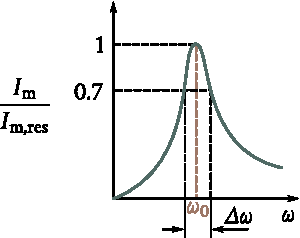
\includegraphics[scale=1]{figures/ch_13/fig_13_9.pdf}
		\caption[]{}
		\label{fig:13_9}
	\end{center}
	\vspace{-0.8cm}
\end{figure}

Lưu ý rằng \eqns{13_43}{13_44} chỉ đúng với các giá trị lớn của $Q$, \ie, khi độ hãm của dao động tự do trong mạch rất nhỏ.

Hiện tượng cộng hưởng được sử dụng để tách các thành phần cần thiết khỏi một điện áp phức tạp.
Giả sử rằng điện áp trên một mạch là
\begin{equation*}
    U = \ab{U}{m,$1$} \cos(\omega_1 t + \alpha_1) + \ab{U}{m,$2$} \cos(\omega_2 t + \alpha_2) + \ldots.
\end{equation*}

\noindent
Bằng cách đưa mạch về các tần số $\omega_1$, $\omega_2$, etc. (\ie, bằng cách chọn các thông số $C$ và $L$ phù hợp), ta có thể nhận được một điện áp trên tụ gấp giá trị của một thành phần điện áp $Q$ lần trong khi điện áp trên tụ do các thành phần điện áp khác sẽ yếu hơn.
Quá trình này diễn ra, chẳng hạn như, khi chỉnh một đài radio đến tần số phù hợp

\section{Dòng điện xoay chiều}\label{sec:13_5}

Dao động tĩnh cưỡng bức ở trên có thể được xem như dòng điện xoay chiều sinh ra bởi điện áp xoay chiều
\vspace{-12pt}
\begin{equation}\label{eq:13_45}
    U = \ab{U}{m} \cos(\omega t)
\end{equation}

\noindent
trong một mạch gồm một tụ, một cuộn cảm và một điện trở.
Theo phương trình \eqref{eq:13_31}, \eqref{eq:13_32} và \eqref{eq:13_33}, dòng này biến thiên theo định luật
\begin{equation}\label{eq:13_46}
    I = \ab{I}{m} \cos(\omega t - \varphi).
\end{equation}

\noindent
Biên độ dòng điện được xác định bởi biên độ điện áp, các thông số mạch $C$, $L$, $R$ và tần số $\omega$:
\begin{equation}\label{eq:13_47}
    \ab{I}{m} = \frac{\ab{U}{m}}{\sqrt{R^2+[\omega L - 1/(\omega C)]^2}}.
\end{equation}

\noindent
Dòng điện trễ pha so với điện áp một góc $\varphi$ phụ thuộc vào các thông số mạch và tần số như sau:
\begin{equation}\label{eq:13_48}
    \tan\varphi = \frac{\omega L - 1/(\omega C)}{R}.
\end{equation}

\noindent
Khi $\varphi<0$, dòng điện thực tế sẽ sớm pha so với điện áp.

Biểu thức
\begin{equation}\label{eq:13_49}
    Z = \parenthesis{R^2 + \parenthesis{\omega L - \frac{1}{\omega C}}^2}^{1/2}
\end{equation}

\noindent
tại tử số của \eqn{13_47} được gọi là \textbf{trở kháng}.

Nếu một mạch chỉ chứa điện trở R $R$, biểu thức cho định luật Ohm có dạng
\begin{equation*}
    IR = \ab{U}{m} \cos(\omega t).
\end{equation*}

\noindent
Do đó, dòng điện trong trường hợp này biến thiên đồng pha với điện áp, với biên độ là
\begin{equation*}
    \ab{I}{m} = \frac{\ab{U}{m}}{R}.
\end{equation*}

\noindent
Khi đối chiếu biểu thức này với \eqn{13_47} cho thấy rằng để một tụ có thể được coi như ngắn mạch thì thì cần tiến đến $C\to\infty$ thay vì tới $C = 0$.

Bất kỳ mạch trên thực tế nào đều có các giá trị hữu hạn của $R$, $L$, và $C$.
Có thể xảy ra các trường hợp mà một vài thông số mạch có giá trị thích hợp để ảnh hưởng lên mạch có thể bỏ qua.
Giả sử rằng giá trị $R$ của một mạch có thể coi như bằng không và $C$ bằng vô cùng.
Từ \eqns{13_47}{13_48} ta có thể thấy rằng
\begin{equation}\label{eq:13_50}
    \ab{I}{m} = \frac{\ab{U}{m}}{\omega L}
\end{equation}

\noindent
và từ đó $\tan\varphi=\infty$ (do đó, $\varphi=\pi/2$).
Đại lượng
\begin{equation}\label{eq:13_51}
    X_L = \omega L
\end{equation}

\noindent
được gọi là \textbf{cảm kháng}.
Nếu $L$ được biểu diễn theo henry và $\omega$ theo \si{\radian\per\second}, khi đó $X_L$ được biểu diễn theo ohm.
Khi khảo sát \eqn{13_51} ta nhận thấy cảm kháng tỉ lệ thuận với tần số $\omega$.
Một cuộn cảm sẽ không có cảm ứng đối với một dòng điện không đổi ($\omega=0$), \ie, $X_L=0$.

Dòng điện trong một cuộn cảm trễ pha so với điện áp một lượng $\pi/2$.
Hay có thể nói, điện áp trên cuộn cảm sớm pha so với dòng điện một lượng $\pi/2$ (xem \fig{13_6}).

Bây giờ, hãy giả thiết rằng cả $R$ và $L$ đều bằng không.
Theo \eqns{13_47}{13_48}, ta có
\begin{equation}\label{eq:13_52}
    \ab{I}{m} = \frac{\ab{U}{m}}{1/(\omega C)}
\end{equation}

\noindent
$\tan\varphi=-\infty$ (\ie, $\varphi=-\pi/2$).
Đại lượng
\begin{equation}\label{eq:13_53}
    X_C = \frac{1}{\omega C}
\end{equation}

\noindent
được gọi là \textbf{dung kháng}.
Nếu $C$ được biểu diễn theo farad, $\omega$ theo \si{\radian\per\second} thì $X_C$ sẽ được biểu diễn theo ohm.
Từ \eqn{13_53} cho thấy rằng dung kháng tỉ lệ nghịch với tần số.
Với một dòng không đổi, $X_C=\infty$---dòng không đổi không thể chạy qua một tụ điện.
Do $\varphi=-\pi/2$, dòng điện qua tụ sớm pha so với điện áp một lượng $\pi/2$.
Hay nói cách khác, điện áp trên tụ trễ pha so với dòng một lượng $\pi/2$ (xem \fig{13_6}).

Cuối cùng, giả thiết rằng $R$ bằng không.
Trong trường hợp này, \eqn{13_47} trở thành
\begin{equation}\label{eq:13_54}
    \ab{I}{m} = \frac{\ab{U}{m}}{|\omega L - 1/(\omega C)|}.
\end{equation}

\noindent
Đại lượng
\begin{equation}\label{eq:13_55}
    X = \omega L - \frac{1}{\omega C} = X_L - X_C
\end{equation}

\noindent
được gọi là \textbf{reactance}.

Phương trình \eqref{eq:13_48} và \eqref{eq:13_49} có thể được viết dưới dạng
\begin{equation*}
    \tan\varphi = \frac{X}{R},\quad Z = \sqrt{R^2+X^2}.
\end{equation*}

\noindent
Do đó, nếu ta có mọt tam giác vuông có hai cạnh bên độ dài bằng giá trị của điện trở $R$ và reactance $X$ thì độ dài của cạnh huyền sẽ có giá trị bằng $Z$ (theo \fig{13_6}).

Hãy tìm năng lượng được giải phóng trong một mạch điện xoay chiều.
Giá trị tức thời của công suất bằng tích của giá trị tức thời của điện áp và dòng điện:
\begin{equation}\label{eq:13_56}
    P(t) = U(t)I(t) = \ab{U}{m} \cos(\omega t) \times \ab{I}{m} \cos(\omega t - \varphi).
\end{equation}

\noindent
Sử dụng đẳng thức lượng giác
\begin{equation*}
    \cos\alpha\cos\beta = \frac{1}{2}\cos(\alpha-\beta) + \frac{1}{2} \cos(\alpha+\beta),
\end{equation*}

\noindent
Ta có thể viết \eqn{13_56} dưới dạng
\begin{equation}\label{eq:13_57}
    P(t) = \frac{1}{2} \ab{U}{m} \ab{I}{m} \cos\varphi + \frac{1}{2} \ab{U}{m} \ab{I}{m} \cos(2\omega t - \varphi).
\end{equation}

Khi tính toán thực tế, ta chỉ quan tâm đến giá trị trung bình của $P(t)$, được ký hiệu bởi $P$.
Do giá trị trung bình của $\cos(2\omega t - \varphi)$ bằng không, ta có
\begin{equation}\label{eq:13_58}
    P = \frac{\ab{U}{m} \ab{I}{m}}{2} \cos\varphi.
\end{equation}

\noindent
Khảo sát \eqn{13_57} cho thấy công suất tức thời biến thiên quanh giá trị trung bình với tần số gấp đôi dòng điện. (\fig{13_10}).

\begin{figure}[t]
	\begin{center}
		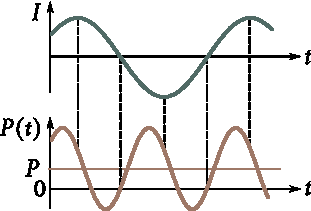
\includegraphics[scale=1]{figures/ch_13/fig_13_10.pdf}
		\caption[]{}
		\label{fig:13_10}
	\end{center}
	\vspace{-0.8cm}
\end{figure}

Theo \eqn{13_48},
\begin{equation}\label{eq:13_59}
    \cos\varphi = \frac{R}{\sqrt{R^2+[\omega L - 1/(\omega C)]^2}} = \frac{R}{Z}.
\end{equation}

\noindent
Sử dụng giá trị  $\cos\varphi$ tại \eqn{13_48} và chú ý rằng $\ab{U}{m}/Z=\ab{I}{m}$, ta được
\begin{equation}\label{eq:13_60}
    P = \frac{R\ab{I}{m}^2}{2}.
\end{equation}

\noindent
Ta có thể thu được công suất này với một dòng điện một chiều độ lớn
\begin{equation}\label{eq:13_61}
    I = \frac{\ab{I}{m}}{\sqrt{2}}.
\end{equation}

\noindent
Đại lượng \eqref{eq:13_61} được gọi là \textbf{giá trị hiệu dụng của dòng điện}.
Tương tự, đại lượng
\begin{equation}\label{eq:13_62}
    U = \frac{\ab{U}{m}}{\sqrt{2}},
\end{equation}

\noindent
được gọi là \textbf{điện áp hiệu dụng}.

Biểu diễn công suất trung bình theo dòng điện và điện áp hiệu dụng, ta được
\begin{equation}\label{eq:13_63}
    P = U I \cos\varphi.
\end{equation}

\noindent
Hệ số $\cos\varphi$ trong biểu thức được gọi là \textbf{power factor}.
Kỹ sư khi thiết kế mạch sẽ tìm cách khiến $\cos\varphi$ cao nhất có thể.
Ở các giá trị nhỏ của $\cos\varphi$, phải cung cấp một dòng lớn để đạt được công suất yêu cầu, và điều này dẫn đến thất thoát lớn ở các đường truyền tải điện.